\documentclass[./main.tex]{subfiles}

\begin{document}

\chapter{Clock calibration}
A TDMA system needs a node to send the synchronization packet, so the rests received those packet able to figure out the right slots send or listen for the network data packet. Therefore, the synchronize packet is also called the clock calibration packet.

When a node joint in a synchronized network, it can take one of the flowing roles:
\begin{itemize}
    \item \textbf{master} (CCP\_ROLE\_MASTER): There is only one master in a network.
    \item \textbf{slave} (CCP\_ROLE\_SLAVE): Slave node receive clock calibration packet and process to send or listen for the packet at a reasonable time.
    \item \textbf{relay} (CCP\_ROLE\_RELAY): Relay node will relay clock calibration packet each time it receives a different one. The main purpose of a relay node is to extend net network coverage.
\end{itemize}

To initialize the system, at least one of the nodes must be configured as a master. The master node will start and control the network and allow other nodes to join and form a network. It is possible to configure more than one node as master, but only one will be active and the others will take the role of slave and/or replay node. A node can take the slave and relay roles at the same time.

\say{\textbf{cpp}} is clock calibration package supplies synchronized network service for the tdma service.

Figure \ref{fig:State diagram of master enabled devices} shows the state diagram of master enabled devices. Every master enabled device begins by entering the slave role. If there is no master in the network, the slave node will not receive any ccp packet. Then, when time is up, that node will change to the master role. It is a case when more than two nodes accept themselves as a master. In this situation, the node with the lowest MAC address is allowed to continue to be master, others will return slave mode.

\begin{figure}[ht]
    \begin{center}
        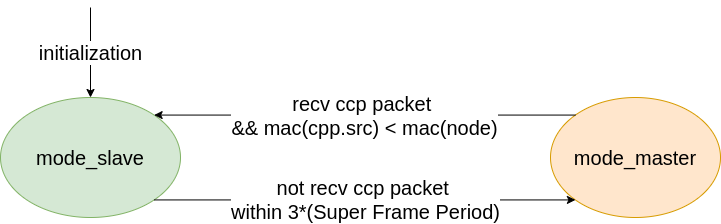
\includegraphics[scale=0.4]{master_enable_device}
    \end{center}
    \caption{State diagram of master enabled devices}
    \label{fig:State diagram of master enabled devices}
\end{figure}

In the implementation, the clock calibration packet is called uwb\_ccp\_blink\_frame\_t as demonstrated in table \ref{tab:uwb_ccp_blink_frame_t}. The size of IEEE 802.15.4e standard blink frame is a 10-byte frame ($+$2 bytes FSC if it is standalone) composed of the fields illustrated in table \ref{tab:IEEE 802.15.4e standard blink}.

\begin{table}[ht]
    \centering
    \begin{tabular}{|g|w|g|w|}
        \rowcolor{LightCyan}
        \hline
        Octets: 1 & 1 & 8 \\ 
        \hline
        fctrl & seq\_num & long\_address/euid \\ 
        \hline
    \end{tabular}
    \caption{ieee\_blink\_frame\_t}
    \label{tab:IEEE 802.15.4e standard blink}
\end{table}

\begin{table}[ht]
    \centering
    \begin{tabular}{|g|w|g|w|}
        \rowcolor{LightCyan}
        \hline
        Octets: 10 & 2 & 8 & 8 \\ 
        \hline
        ieee\_blink\_frame\_t & short\_address & transmission\_interval & transmission\_timestamp \\ 
        \hline
        \rowcolor{LightCyan}
        1 & 1 & 2 & \\
        \hline
        rpt\_count & rpt\_max & epoch\_to\_rm\_us & \\
        \hline
    \end{tabular}
    \caption{uwb\_ccp\_blink\_frame\_t}
    \label{tab:uwb_ccp_blink_frame_t}
\end{table}

\end{document}